\chapter{Nuclear Uncertainties}
\section{Introduction}
%
In this chapter we address another important source of theory uncertainty in PDFs. This arises because in order to maximally constrain them, PDFs are determined by fitting a range of experimental data over a wide variety of processes. Some of this data consists of measurements on nuclear targets, rather than proton targets. In this case, the surrounding nuclear environment will have an effect on the measured observables, which in turn will influence the form of the fitted PDFs. The uncertainties associated with these effects are termed "nuclear uncertainties". Such uncertainties are small \cite{Ball:2009mk}\cite{Ball:2013gsa} but becoming increasingly relevant with the advent of the Large Hadron Collider and the era of precision physics it has ushered in \cite{Gao:2017yyd}.

Here we show how to use existing nuclear PDFs (nPDFs) to provide an estimate of nuclear uncertainties, and include them in future proton PDF fits within the Neural Network PDF (NNPDF) framework \cite{Ball:2008by} \footnote{For a more detailed analysis, see \cite{Ball:2018twp}.}. We first review the nuclear data (Sec. \ref{sec:nucdat}), then outline the construction and form of nuclear uncertainties (Sec. \ref{sec:nucuncs}). Finally, we assess the impact on the PDFs and associated phenomenology (Secs. \ref{sec:impact} and \ref{sec:pheno}).
%
\section{Nuclear Data} \label{sec:nucdat}
%
There are three experiments with nuclear targets currently included in NNPDF analyses: 
charged current inclusive deep inelastic scattering (DIS) cross sections from CHORUS \cite{Onengut:2005kv}, on Pb; DIS dimuon cross sections from NuTeV \cite{Goncharov:2001qe}\cite{Tzanov:2005kr} on Fe; and Drell-Yan dimuon cross sections from E605 at Fermilab \cite{Aaltonen:2008eq}, on Cu. After cuts, nuclear data make up 993/4285 of the data points ($\sim$ 23\%). For a complete summary of the data sets, see \cite{Ball:2017nwa}.

A study of the correlation between these measurements and the fitted PDFs reveals that the CHORUS data has most impact on the up- and down-valence distributions, NuTeV data has most impact on the strange, and E605 data has most impact on the other light sea quarks: anti-up and anti-down. Therefore, we anticipate largest effects from nuclear uncertainties in these PDFs.
%
\section{Determining Nuclear Uncertainties} \label{sec:nucuncs}
%
In a PDF fit we include an experimental covariance matrix, $C_{ij}$, describing the breakdown of statistical and systematic errors, where $i,j$ run over the data points. Uncertainties due to nuclear data must be considered in addition to the experimental uncertainties, and in general they can be encapsulated in a theoretical covariance matrix, $S_{ij}$. In a PDF fit we simply add this to $C_{ij}$ \cite{Ball:2018odr}, so that the nuclear uncertainties act like experimental systematics.

We adopted an empirical approach to construct the nuclear uncertainties, using nPDFs rather than appealing to nuclear models, which rely on various assumptions \cite{Arneodo:1992wf}. We compared theoretical predictions for nuclear observables made with the correct corresponding nPDFs for an isotope ``$N$", $T_i^N[f_N^{(n)}]$, to those with proton PDFs, $T_i^N[f_p]$. Here $f_p$ is the central value for a proton PDF and $f_N^{(n)}$ is one Monte Carlo replica in an nPDF ensemble, where $n = 1, ..., N_{rep}$ \cite{Butterworth:2015oua}. To generate such an ensemble we combined three recent nPDF sets: DSSZ12 \cite{deFlorian:2011fp}, nCTEQ15 \cite{Kovarik:2015cma} and EPPS16 \cite{Eskola:2016oht}. Note that DSSZ12 does not provide a Cu PDF, so for the case of E605 we combined just two nPDF sets.
%%%%%%%%%%%%%%%%%%%%%%%%%%%%%%%%%%%%%%%%%%%%%%%%%%%%%%%%%%%%

We considered two definitions of nuclear uncertainties:
\begin{enumerate}
\item \textbf{Def. 1, }(a conservative approach) where the only modification is to include nuclear uncertianties, with \begin{equation}
\Delta_i^{(n)} = T_i^N[f_N^{(n)}] - T_i^N[f_p];
\end{equation}
\item \textbf{Def. 2, } (a more ambitious approach) where a shift,
\begin{equation}
\delta T_i^N = T_i^N[f_N] - T_i^N[f_p],
\end{equation} 
is also applied to the corresponding observable, meaning that the uncertainty should be defined relative to the shifted value,
\begin{equation}
\Delta_i^{(n)} = T_i^N[f_N^{(n)}] - T_i^N[f_N].
\end{equation}
\end{enumerate}

\begin{figure}
  \centering
  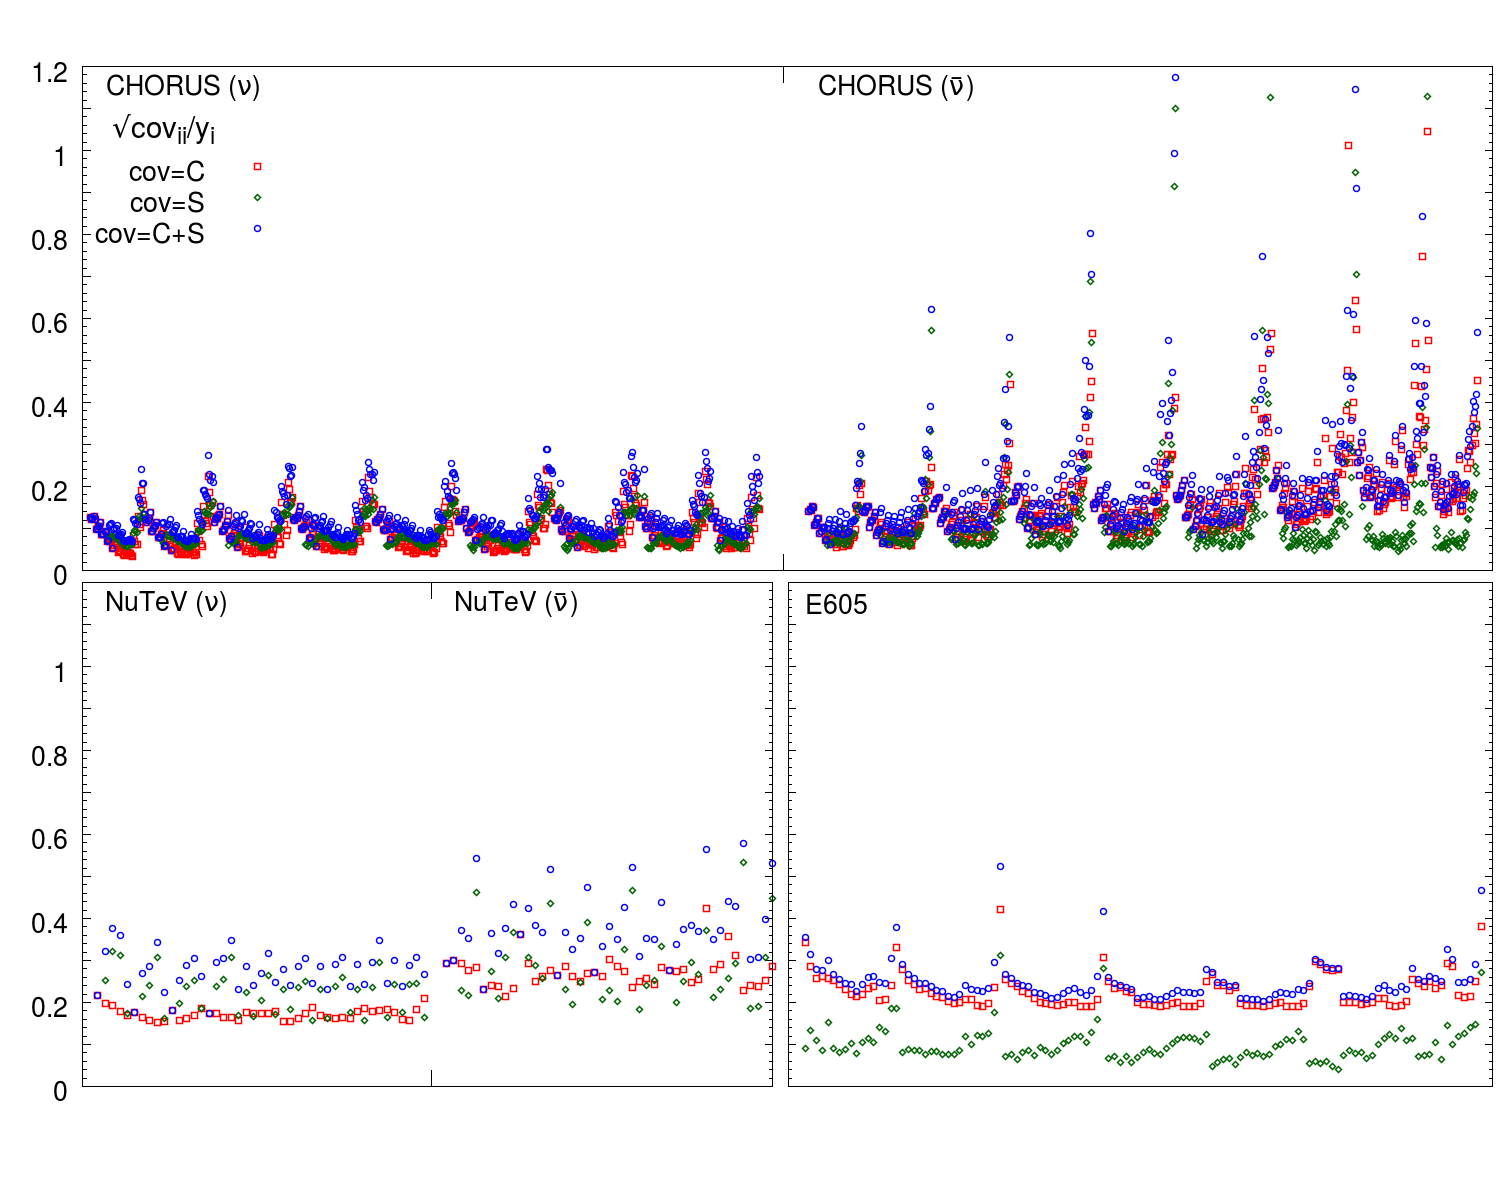
\includegraphics[width=\textwidth]{nuclear/covimpact1.jpg}
    \caption{ The square root of the diagonal elements of the covariance matrices, normalised to corresponding data. Experimental contributions are red, theory green and the total blue. Data from CHORUS and NuTeV are split into neutrino and anti-neutrino parts. Points are binned in (anti-)neutrino beam energy $E$: 25, 35, 45, 55, 70, 90, 110, 120, 170 GeV. In each bin $x$ increases from left to right, 0.045 $< x <$ 0.65.\label{fig:diagcovmat}}
\end{figure}

Whilst Def. 1 just deweights the nuclear data sets in a PDF fit, Def. 2 also attempts to directly apply a nuclear correction. In both cases we can construct a theoretical covariance matrix as
\begin{equation}
S_{ij} = \frac{1}{N_{rep}} \sum_{n=1}^{N_{rep}} \Delta_i^{(n)} \Delta_j^{(n)}.
\end{equation}
We did this separately for each experiment, which is a conservative treatment.

Considering the diagonal elements of the covariance matrices (Fig. \ref{fig:diagcovmat}), we see that the nuclear uncertainty has the largest impact on the NuTeV data, where the nuclear uncertainties dominate the data uncertainties. This is mirrored in the off-diagonal elements (Fig. \ref{fig:corrmats}). Given the high correlation of NuTeV observables with the $s$ and $\bar{s}$ PDFs, the effect of including the uncertainties ought to be greatest for these PDFs.
%
\section{The Impact on Global PDFs} \label{sec:impact}
%
We compared four different PDF fits:
\begin{itemize}
\item \textbf{Baseline, } based on NNPDF3.1, with small improvements \cite{Ball:2018odr};
\item \textbf{NoNuc, } Baseline with nuclear data removed;
\item \textbf{NucUnc, } Baseline with nuclear uncertainties according to Def. 1.
\item \textbf{NucCor, } Baseline with nuclear uncertainties and a nuclear correction according to Def. 2.
\end{itemize}
%%%%%%%%%%%%%%%%%%%%%%%%%%%%%%%%%%%%%%%%%%%%%%%%%%%%%%%%%%%%
\begin{figure} 
  \centering
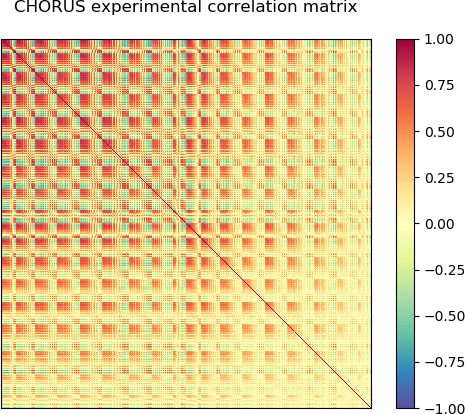
\includegraphics[width=0.45\linewidth]{nuclear/corrplot_exp_CHORUS_def1.png}
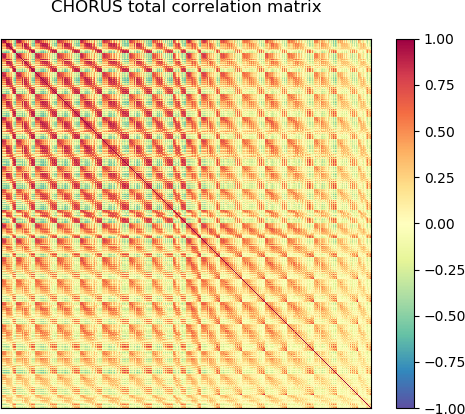
\includegraphics[width=0.45\linewidth]{nuclear/corrplot_tot_CHORUS_def1.png}
\newline
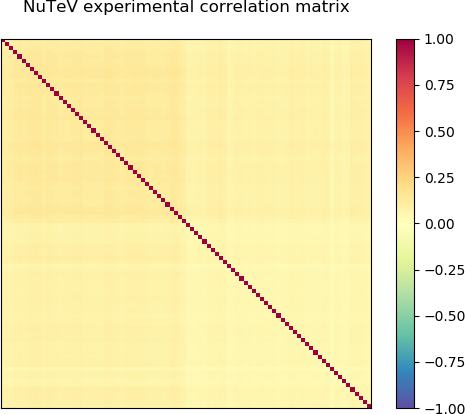
\includegraphics[width=0.45\linewidth]{nuclear/corrplot_exp_NTV_def1.png}
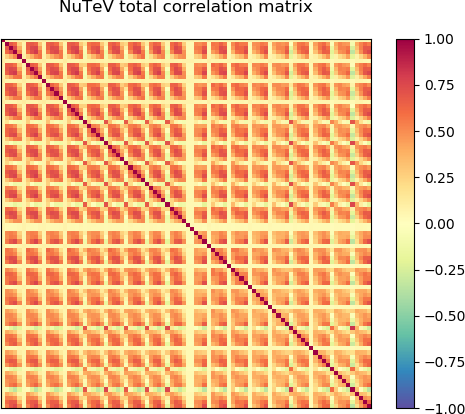
\includegraphics[width=0.45\linewidth]{nuclear/corrplot_tot_NTV_def1.png}
\newline
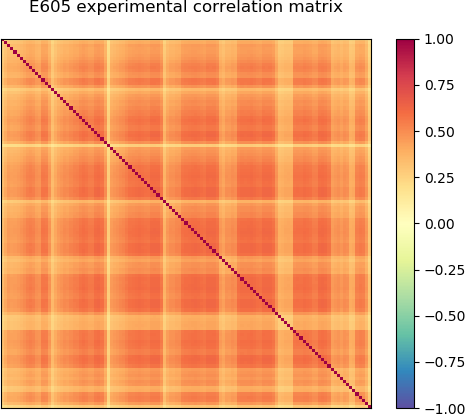
\includegraphics[width=0.45\linewidth]{nuclear/corrplot_exp_DYE605_def1.png}
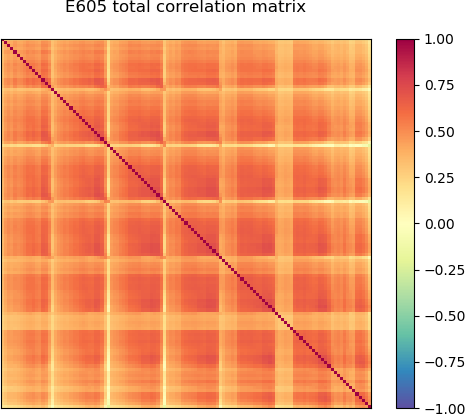
\includegraphics[width=0.45\linewidth]{nuclear/corrplot_tot_DYE605_def1.png}
      \caption{Correlation matrices, $\rho^{cov}_{ij} = \frac{cov_{ij}}{\sqrt{cov_{ii}cov_{jj}}}$, before (left) and after (right) including nuclear uncertainties. Data are binned the same as in Fig. \ref{fig:diagcovmat}. The top row corresponds to CHORUS, middle row to NuTeV and bottom row to E605. Results are displayed for Def. 1 but are qualitatively similar for Def. 2. \label{fig:corrmats}}
\end{figure}
%%%%%%%%%%%%%%%%%%%%%%%%%%%%%%%%%%%%%%%%%%%%%%%%%%%%%%%%%%%%

Table \ref{tab:chi2} shows the variation in $\chi^2$ for selected data sets \footnote{For a full break-down see \cite{Ball:2018odr}.}. All of the fits show reduced $\chi^2$ compared to Baseline, highlighting tension due to nuclear data. However, the strange-sensitive ATLAS $W/Z$ at 7 TeV (2011) measurements \cite{Aad:2011dm} still have a poor $\chi^2$, indicating that possible tensions with NuTeV were unlikely responsible for this; in any case, the data sets occupy different kinematic regions. The best fit is obtained for NucUnc, which has the largest uncertainties.

Fig. \ref{fig:pdfs} shows the light sea quark PDFs for NucUnc compared to Baseline. These are the distributions with greatest impact, but there is little appreciable change other than a small shift in the central value and increase in uncertainties. NucCor behaves similarly. Overall, the nuclear uncertainties are small compared to the global experimental uncertainty.

%%%%%%%%%%%%%%%%%%%%%%%%%%%%%%%%%%%%%%%%%%%%%%%%%%%%%%%%%%%%
\begin{table}
\begin{tabular}{l||l|llll}
Experiment            & $N_{dat}$ & Baseline & NoNuc & NucUnc & NucCor \\
\hline
\hline
CHORUS $\nu$           &  416 & 1.29 & -- & 0.97 & 1.04   \\
CHORUS $\bar{\nu}$    &  416 & 1.20  &  -- & 0.78  & 0.83    \\
NuTeV $\nu$  & 39  & 0.41 & -- & 0.31  & 0.40  \\
NuTeV   $\bar{\nu}$ & 37 & 0.90 & -- &  0.62 & 0.83 \\
E605 $\sigma^p$  &  85 & 1.18 & --  & 0.85 & 0.89 \\
ATLAS $W/Z$ (2011) & 34 & 1.97 & 1.78 & 1.87 & 1.94 \\
ATLAS & 360 & 1.08 & 1.04 & 1.04 & 1.05 \\
CMS & 409 & 1.07 & 1.07 & 1.07 & 1.07 \\
LHCb & 85 & 1.46 & 1.27 & 1.32 & 1.37 \\
\hline
Total & 4285 & 1.18  & 1.14  & 1.07  & 1.09      
\end{tabular}
\caption{$\chi^2$ per data point for selected data sets. The final row shows results for the full fitted data.\label{tab:chi2}}
\end{table}
 
\begin{figure}
  \centering
  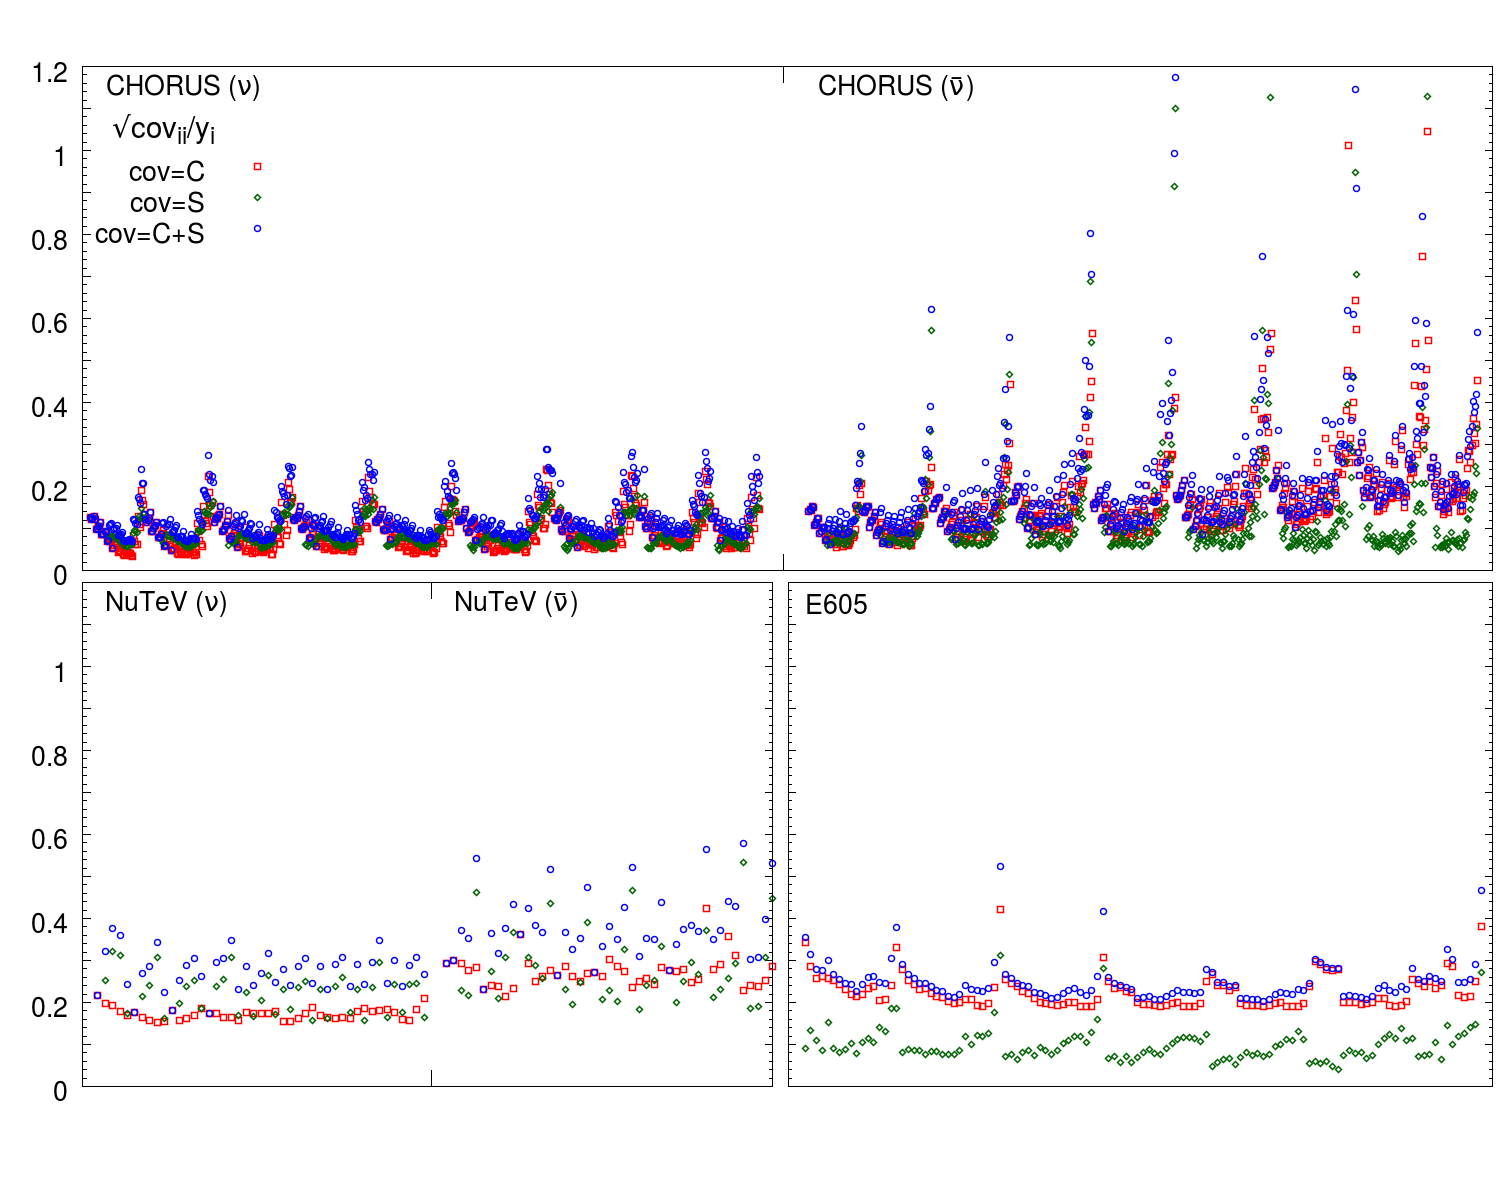
\includegraphics[width=\textwidth]{nuclear/covimpact1.jpg}
    \caption{The square root of the diagonal elements of the covariance matrices, normalised to corresponding data. Experimental contributions are red, theory green and the total blue. Data from CHORUS and NuTeV are split into neutrino and anti-neutrino parts. Points are binned in (anti-)neutrino beam energy $E$: 25, 35, 45, 55, 70, 90, 110, 120, 170 GeV. In each bin $x$ increases from left to right, 0.045 $< x <$ 0.65.\label{fig:diagcovmat}}
\end{figure}
%%%%%%%%%%%%%%%%%%%%%%%%%%%%%%%%%%%%%%%%%%%%%%%%%%%%%%%%%%%%
\section{Phenomenology} \label{sec:pheno}
%
Given the changes to the light sea quark PDFs, it is interesting to examine the impact on relevant phenomenological quantities, namely: the sea quark asymmetry, $\bar{u}/\bar{d}$; strangeness fraction, $R_s = (s+ \bar{s})/(\bar{u} + \bar{d})$; and strange valence distribution, $xs^- = x(s - \bar{s})$ (Fig. \ref{fig:pheno}). In all cases it is clear that removing the nuclear data has a significant effect, emphasising the need to retain this data in proton PDF fits. Adding nuclear uncertainties, however, makes very little difference. In particular, the known tension between ATLAS $W/Z$ + HERA DIS data and NuTeV data, which is apparent in the strangeness fraction \cite{Aad:2012sb}, is not relieved with the addition of nuclear uncertainties. 

%%%%%%%%%%%%%%%%%%%%%%%%%%%%%%%%%%%%%%%%%%%%%%%%%%%%%%%%%%%%
\begin{figure}
  \centering
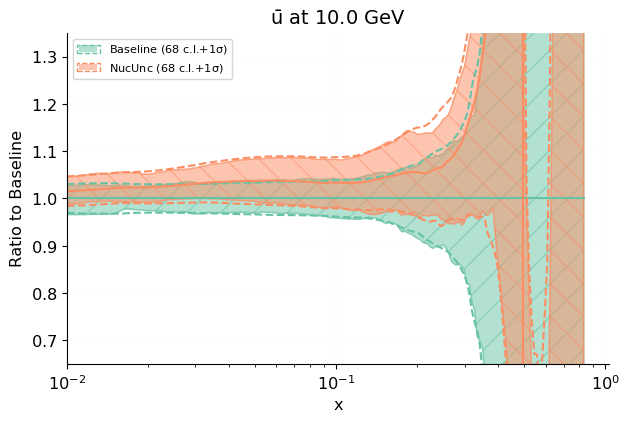
\includegraphics[width=0.45\linewidth]{nuclear/pdf_cv_nucldef1_baru.png}
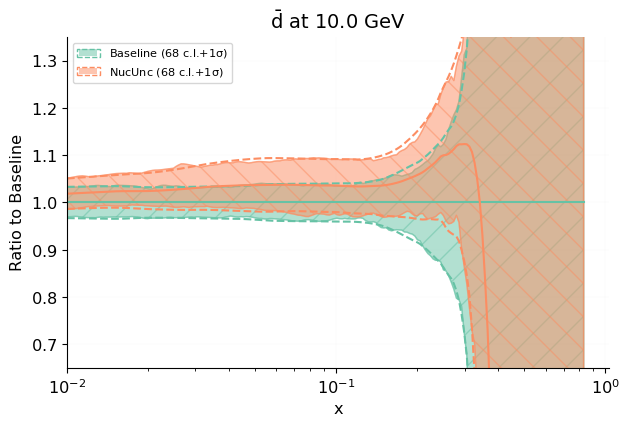
\includegraphics[width=0.45\linewidth]{nuclear/pdf_cv_nucldef1_bard.png}
\newline
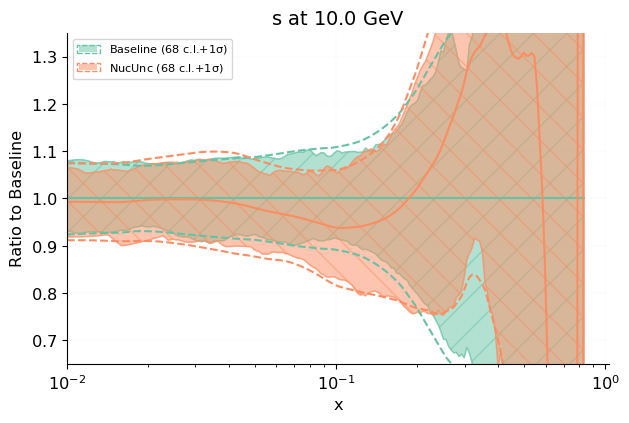
\includegraphics[width=0.45\linewidth]{nuclear/pdf_cv_nucldef1_s.png}
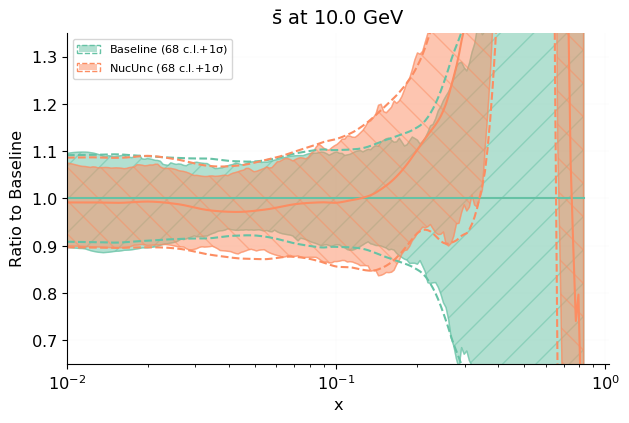
\includegraphics[width=0.45\linewidth]{nuclear/pdf_cv_nucldef1_bars.png}
    \caption{\footnotesize  NucUnc fits with nuclear uncertainties (orange) compared to Baseline (green) for PDFs at 10 GeV. Clockwise from top left: $\bar{u}$, $\bar{d}$, $s$ and $\bar{s}$ PDFs. Error bands are 1 $\sigma$; results are normalised to Baseline fit.  \label{fig:pdfs}}
\end{figure}
%%%%%%%%%%%%%%%%%%%%%%%%%%%%%%%%%%%%%%%%%%%%%%%%%%%%%%%%%%%%
We found no appreciable difference between using NucUnc versus NucCor, so opt to incorporate uncertainties using NucUnc (Def. 1) as this is the more conservative option.

\section{Conclusions} \label{sec:conc}
%
We studied the role of nuclear data in proton PDF fits, and adopted an empirical approach to determine the nuclear uncertainties due to this data. We based our analysis on recent nPDF fits DSSZ12, nCTEQ15 and EPPS16. Using a theoretical covariance matrix, we included these uncertainties in proton PDF fits, and found that the fit quality was improved, with the largest effect on the light sea quark distributions \footnote{The PDF sets from this analysis are available upon request from the authors in LHAPDF format \cite{Buckley:2014ana}.}. We found no significant impact on associated phenomenology. 
%%%%%%%%%%%%%%%%%%%%%%%%%%%%%%%%%%%%%%%%%%%%%%%%%%%%%%%%%%%%
\begin{figure}[h]
  \centering
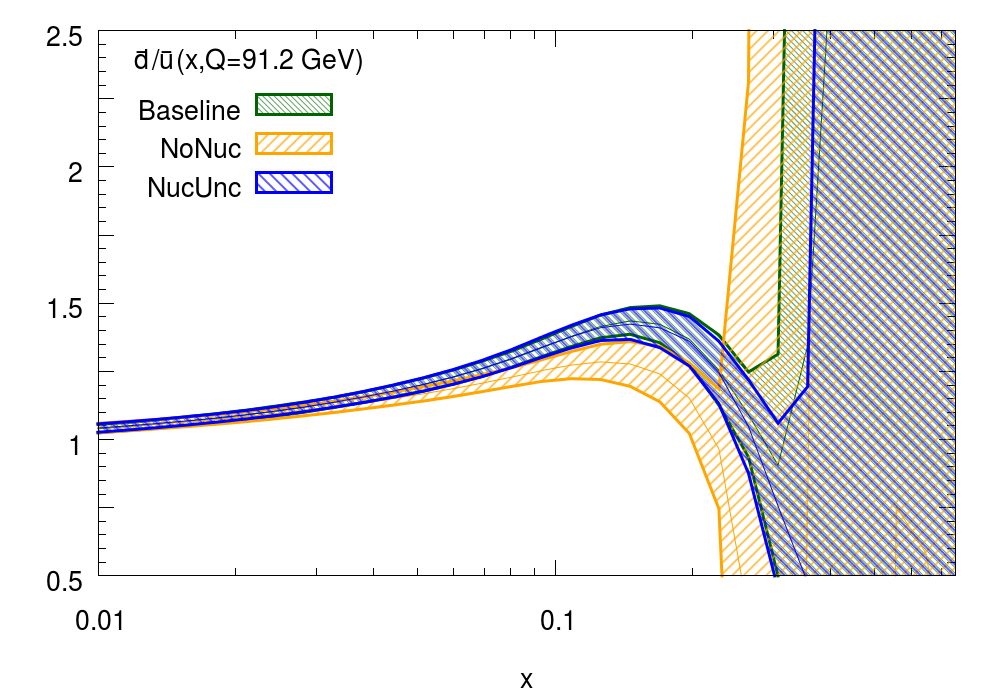
\includegraphics[width=0.6\linewidth]{nuclear/du_max.png}
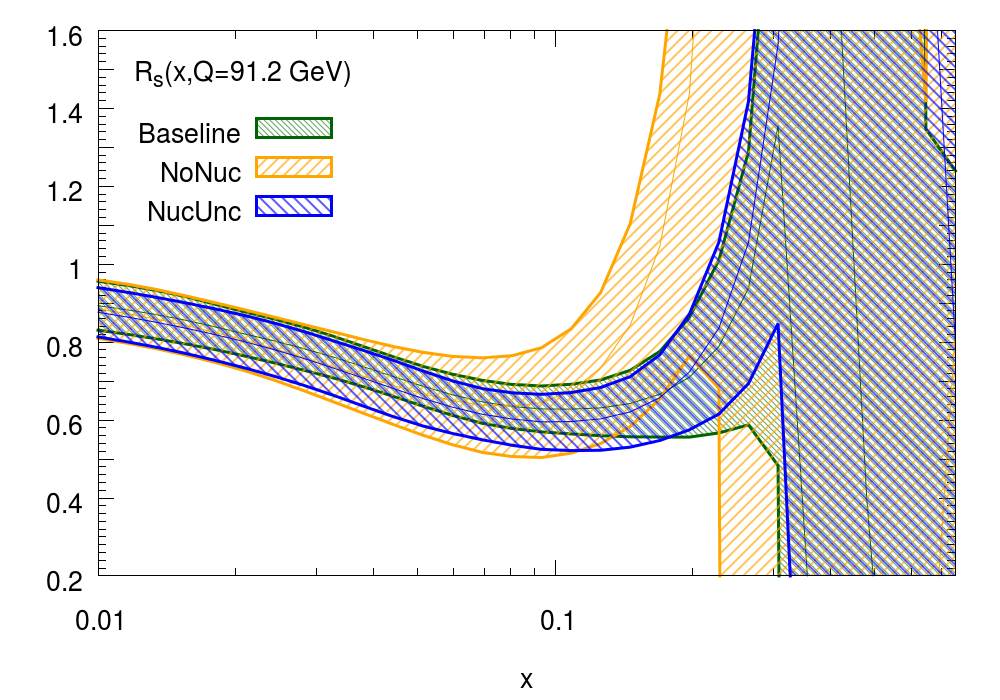
\includegraphics[width=0.6\linewidth]{nuclear/Rs_max.png}
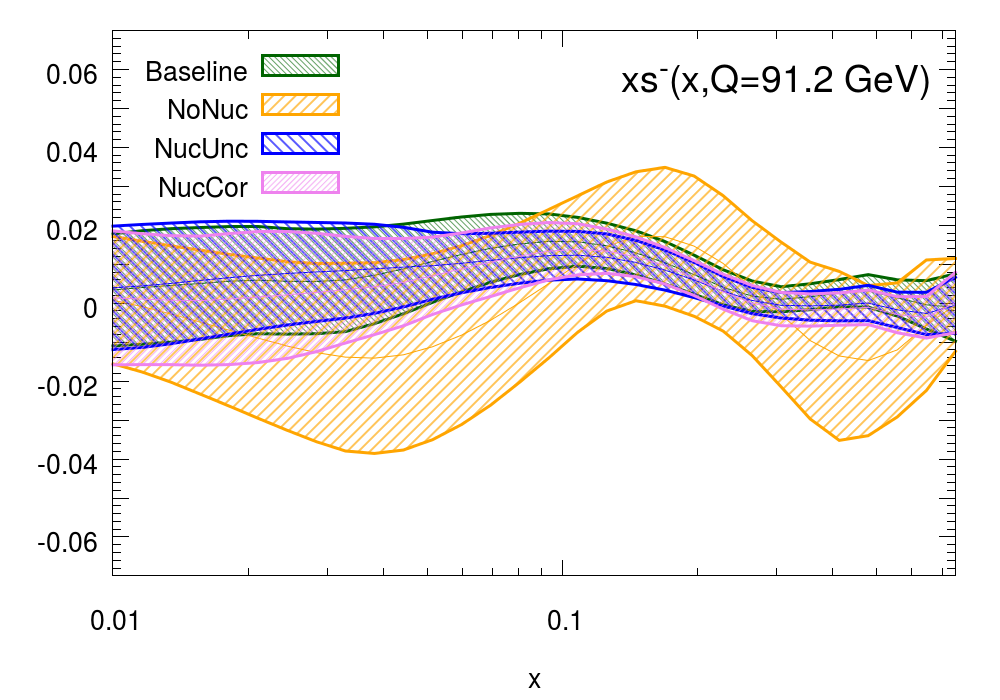
\includegraphics[width=0.6\linewidth]{nuclear/sval_max.png}
    \caption{Effect of including nuclear uncertainties on phenomenology. From left to right: sea quark asymmetry, strangeness fraction, strange valence distribution. Distributions correspond to the use of different PDF fits: Baseline (green), NoNuc (yellow), NucUnc (blue) and NucCor(pink). $Q$ = 91.2 GeV. In the left two plots, NucCor are indistinguishable from NucUnc so are omitted for readability.\label{fig:pheno}} 
\end{figure}
%%%%%%%%%%%%%%%%%%%%%%%%%%%%%%%%%%%%%%%%%%%%%%%%%%%%%%%%%%%%

We will extend this analysis to deterium data, and in the future we will be able to use nuclear PDFs from NNPDF \cite{Khalek:2018bbv} to estimate uncertainties. Furthermore, these methods can be applied to other sources of theoretical uncertainties, such as higher twist effects, fragmentation functions, and missing higher order uncertainties \cite{AbdulKhalek:2019bux}.
